\section{Diagramas de classe do GOD}


\subsection{GOD}
% \begin{figure}
% \caption{Diagrama do GOD}
% \centering
% \includegraphics[\linewidth]{figures/GOD.png}
% \label{fig:god}
% \end{figure}


\subsection{Banco de dados (GODBases)}

\begin{figure}[H]
\centering
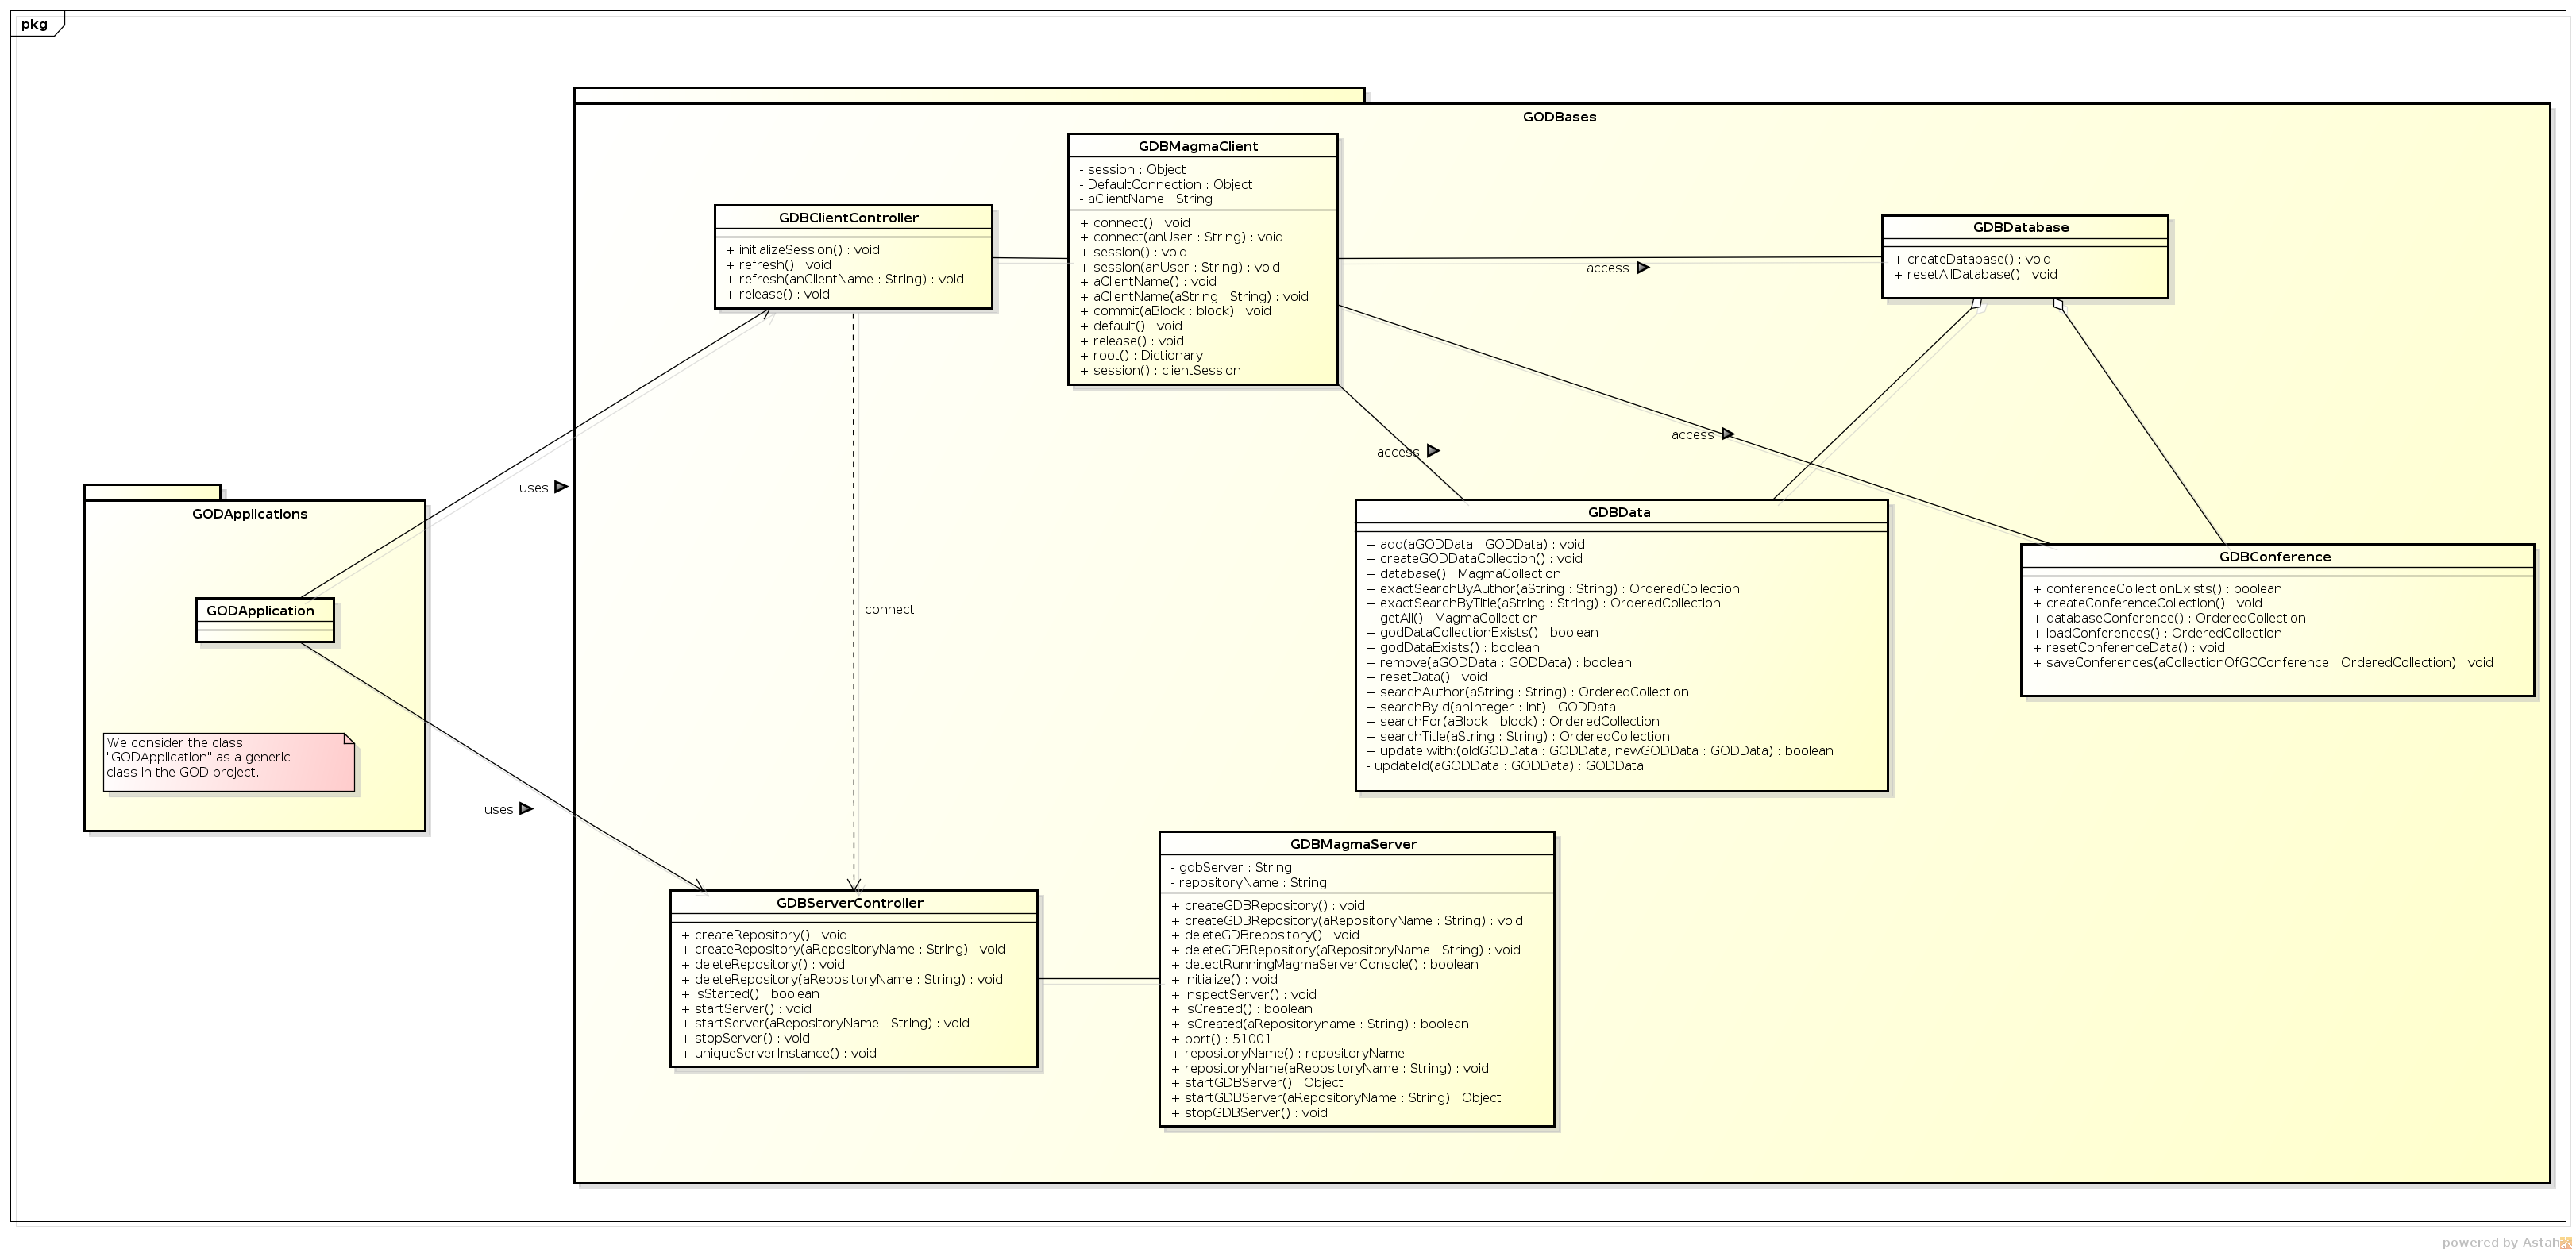
\includegraphics[width=\linewidth]{cd_GODBases.png}
\label{fig:cd-godbases}
\end{figure}

\subsection{E-mails (GODEmail)}
\begin{figure}[H]
\centering
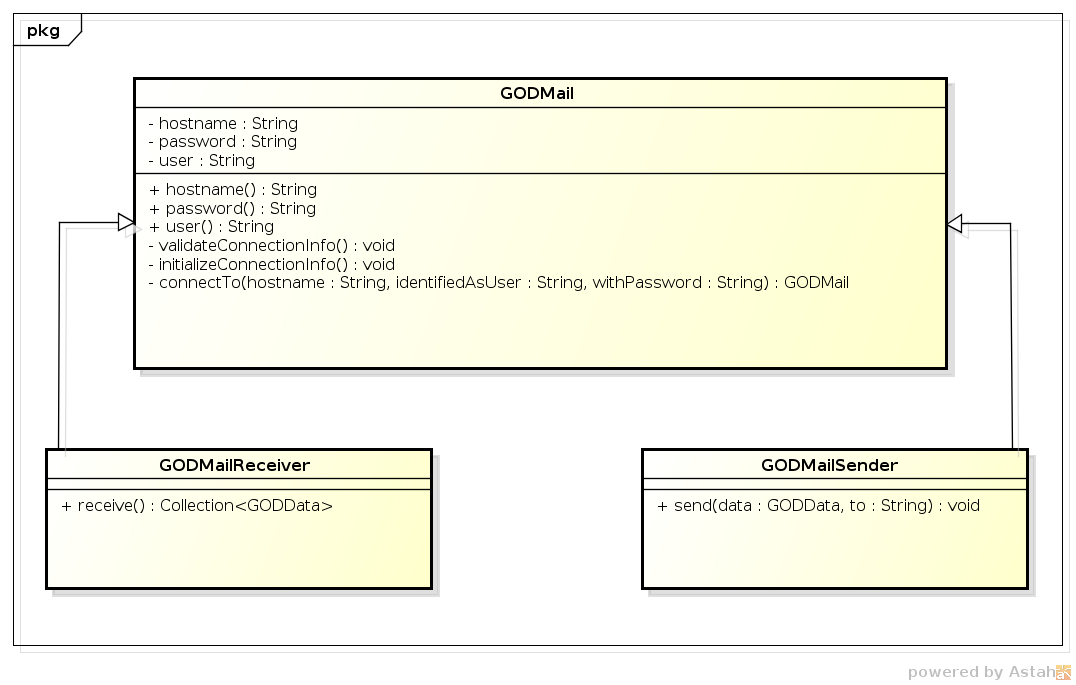
\includegraphics[width=\linewidth]{cd_GODEmail.png}
\label{fig:cd-godemail}
\end{figure}

\subsection{Filtros (GODFilter)}
\begin{figure}[H]
\centering
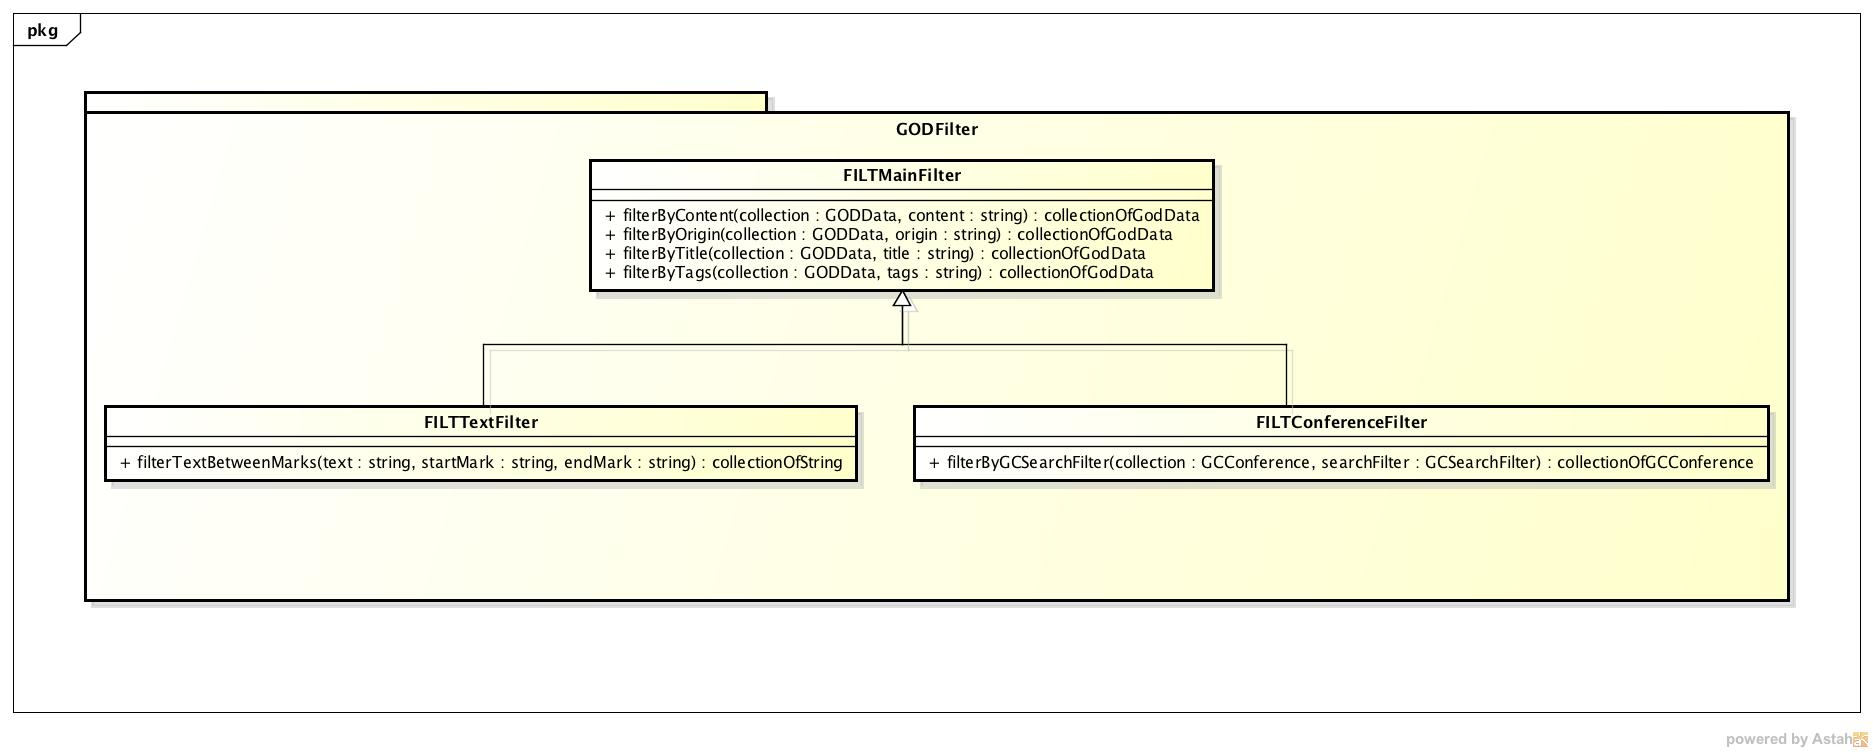
\includegraphics[width=\linewidth]{cd_GODFilter.jpg}
\label{fig:cd-godfilter}
\end{figure}

\subsection{Gráficos (GODGraphGenerator)}
\begin{figure}[H]
\centering
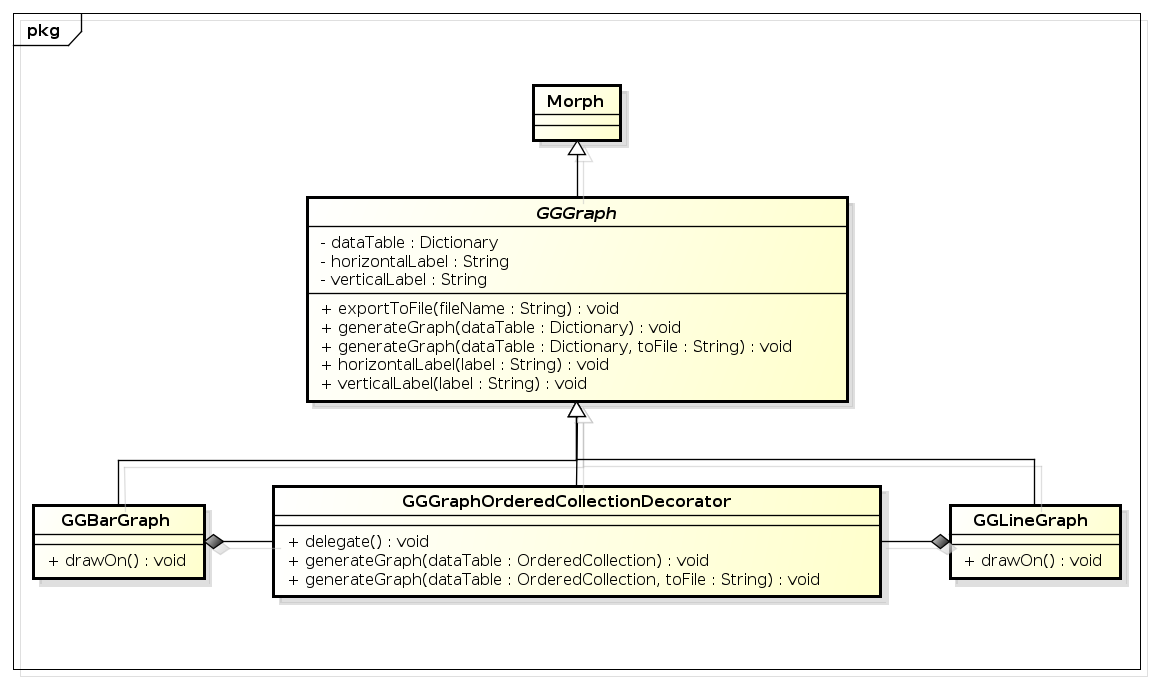
\includegraphics[width=\linewidth]{cd_GODGraphGenerator.png}
\label{fig:cd-godgraphgenerator}
\end{figure}

\subsection{Planilhas (GODSpreadsheet)}
\begin{figure}[H]
\centering
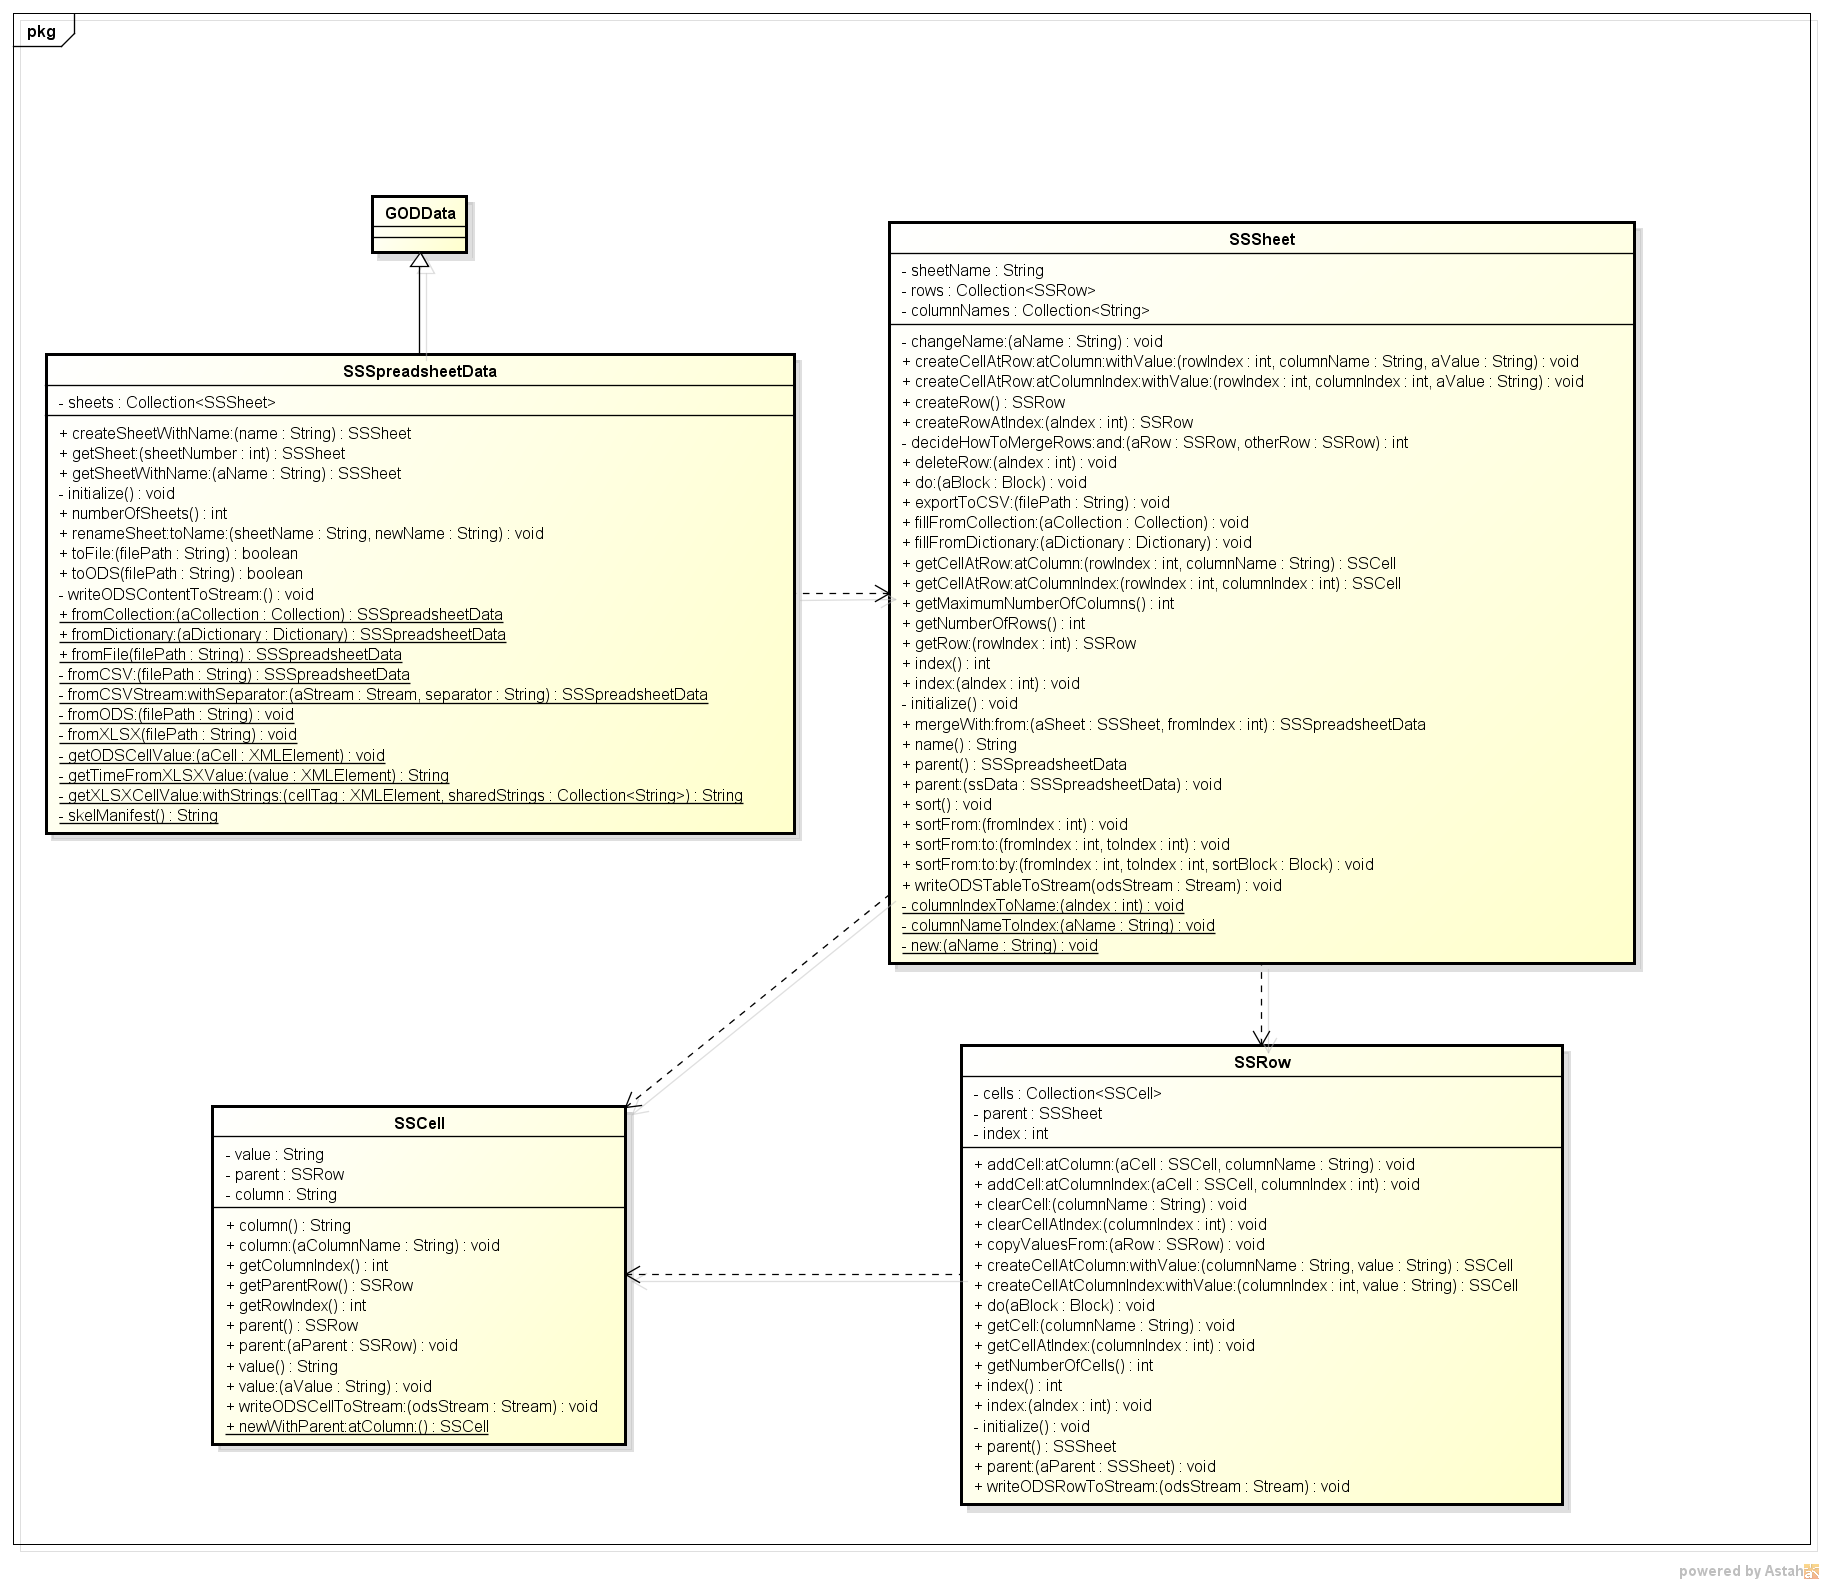
\includegraphics[width=\linewidth]{cd_GODSpreadsheet.png}
\label{fig:cd-godspreadsheet}
\end{figure}

\subsection{Processadores (GODProcessors)}
\begin{figure}[H]
\centering
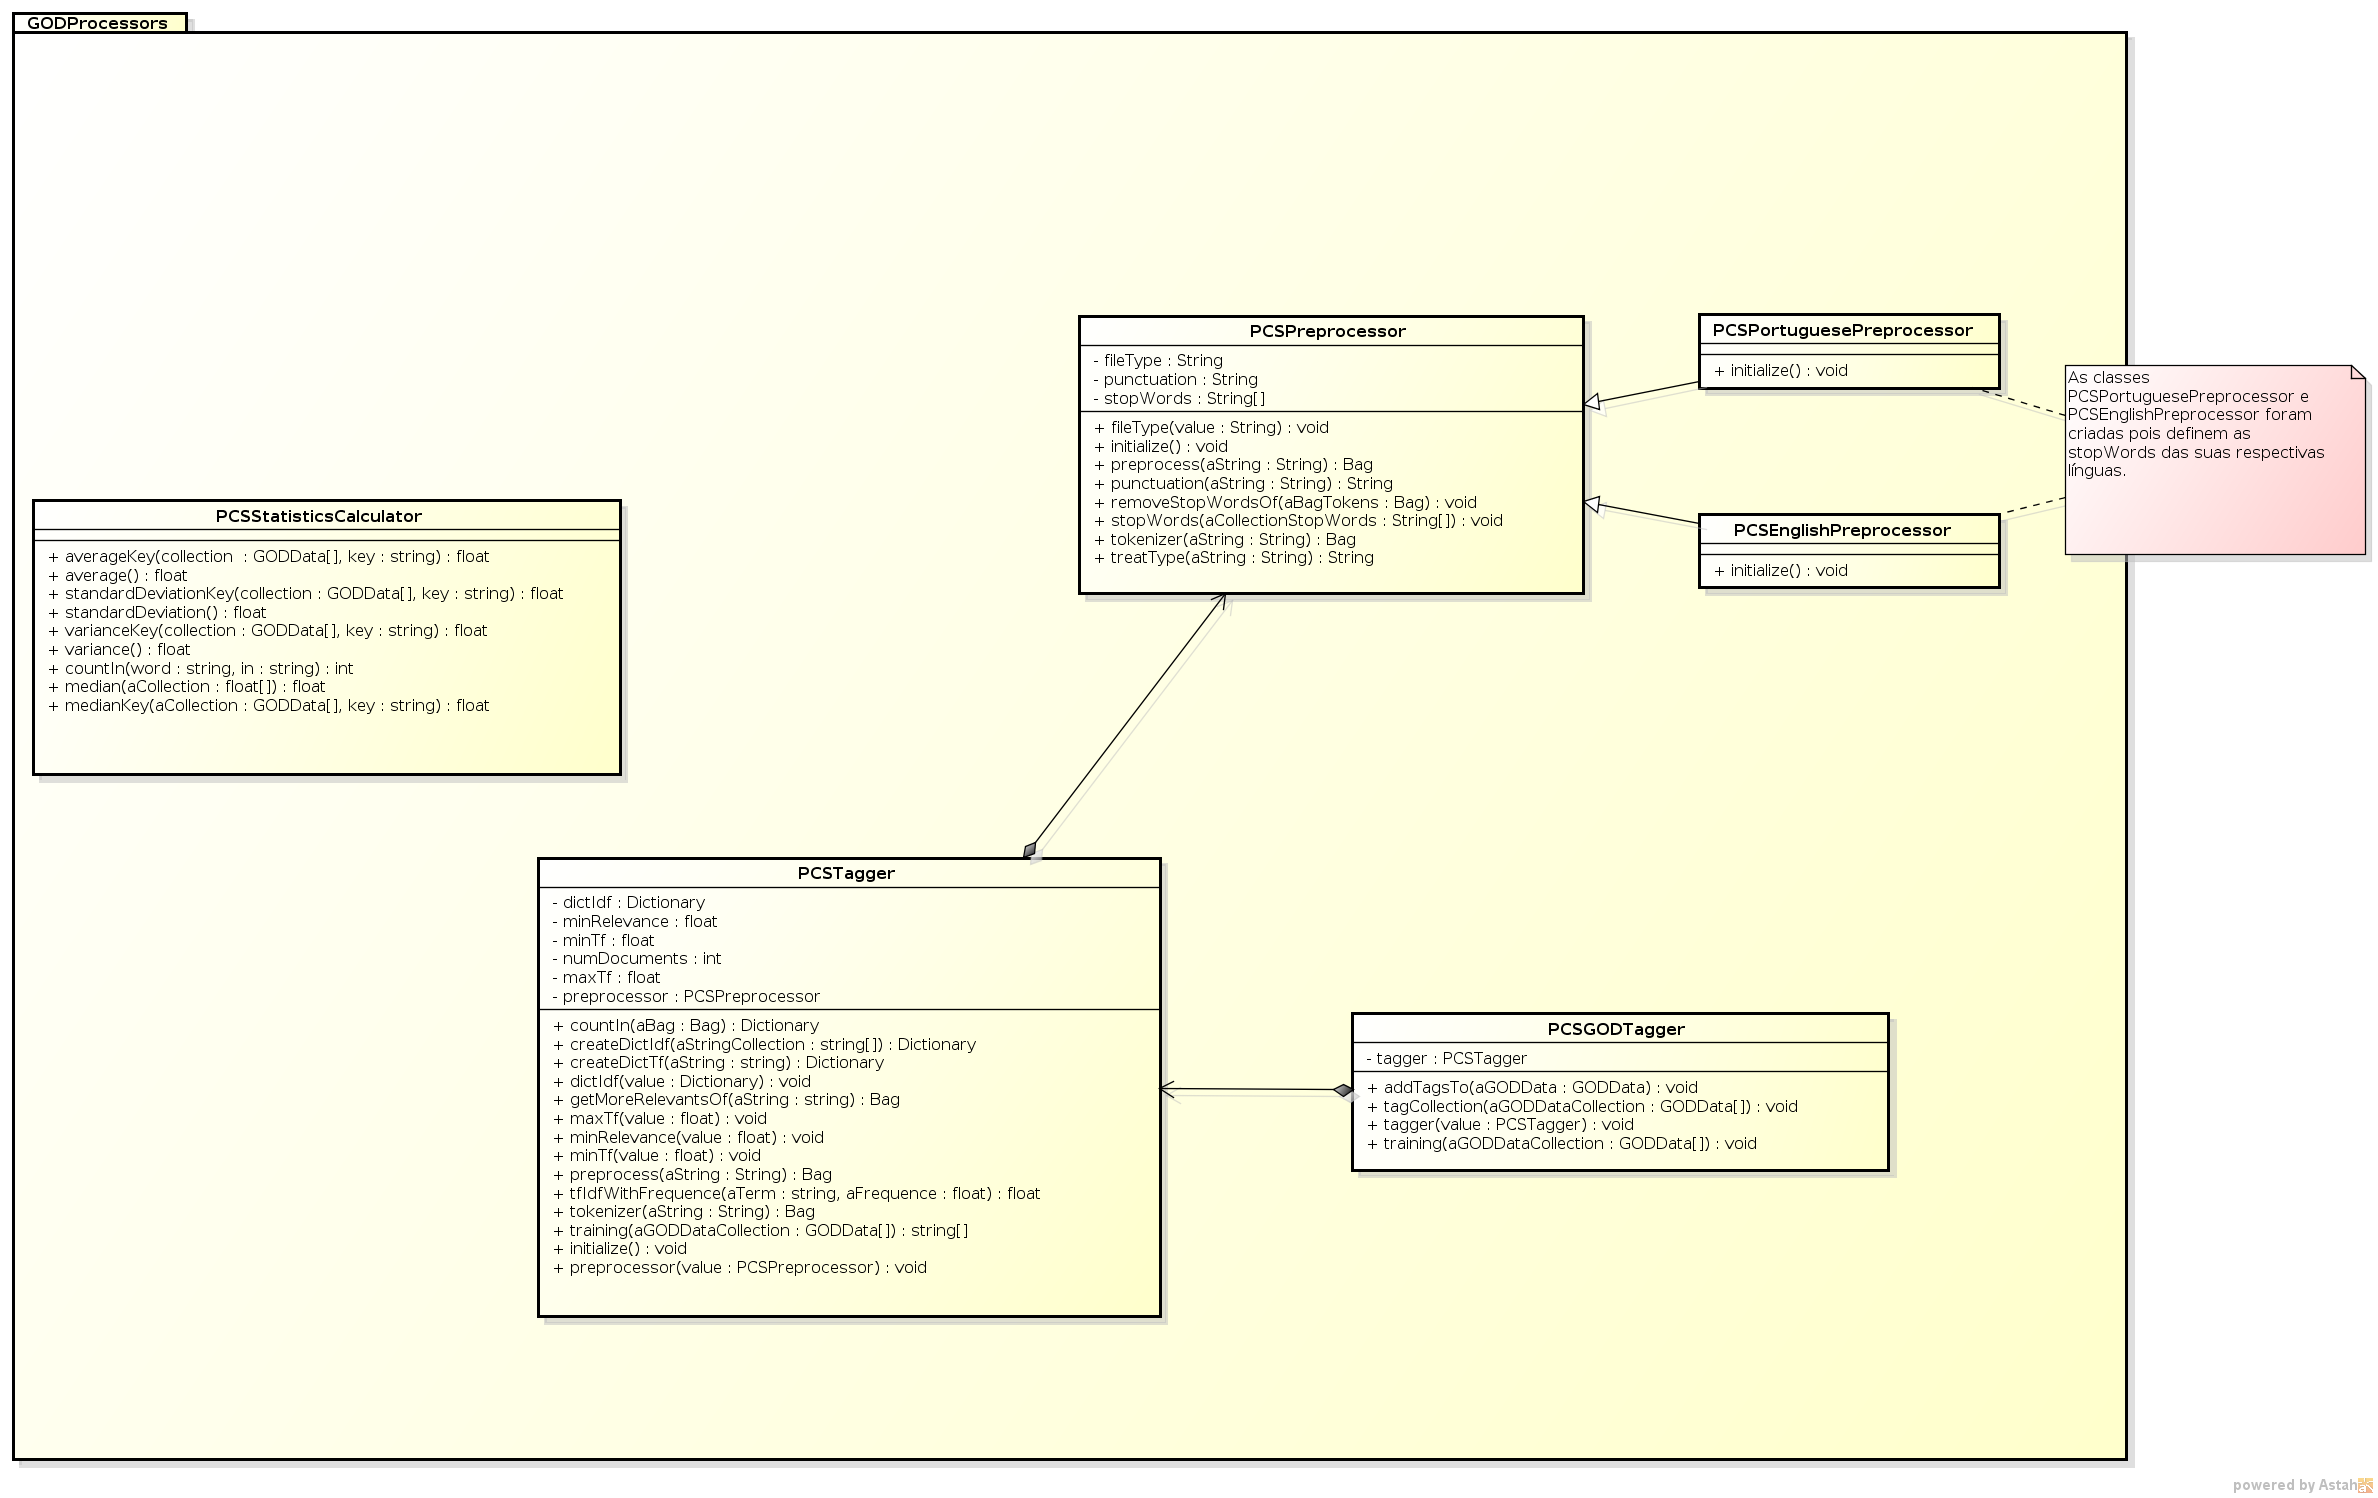
\includegraphics[width=\linewidth]{cd_GODProcessors.png}
\label{fig:cd-godprocessors}
\end{figure}

\subsection{Redes sociais (GODSocialNetIO)}
\begin{figure}[H]
\centering
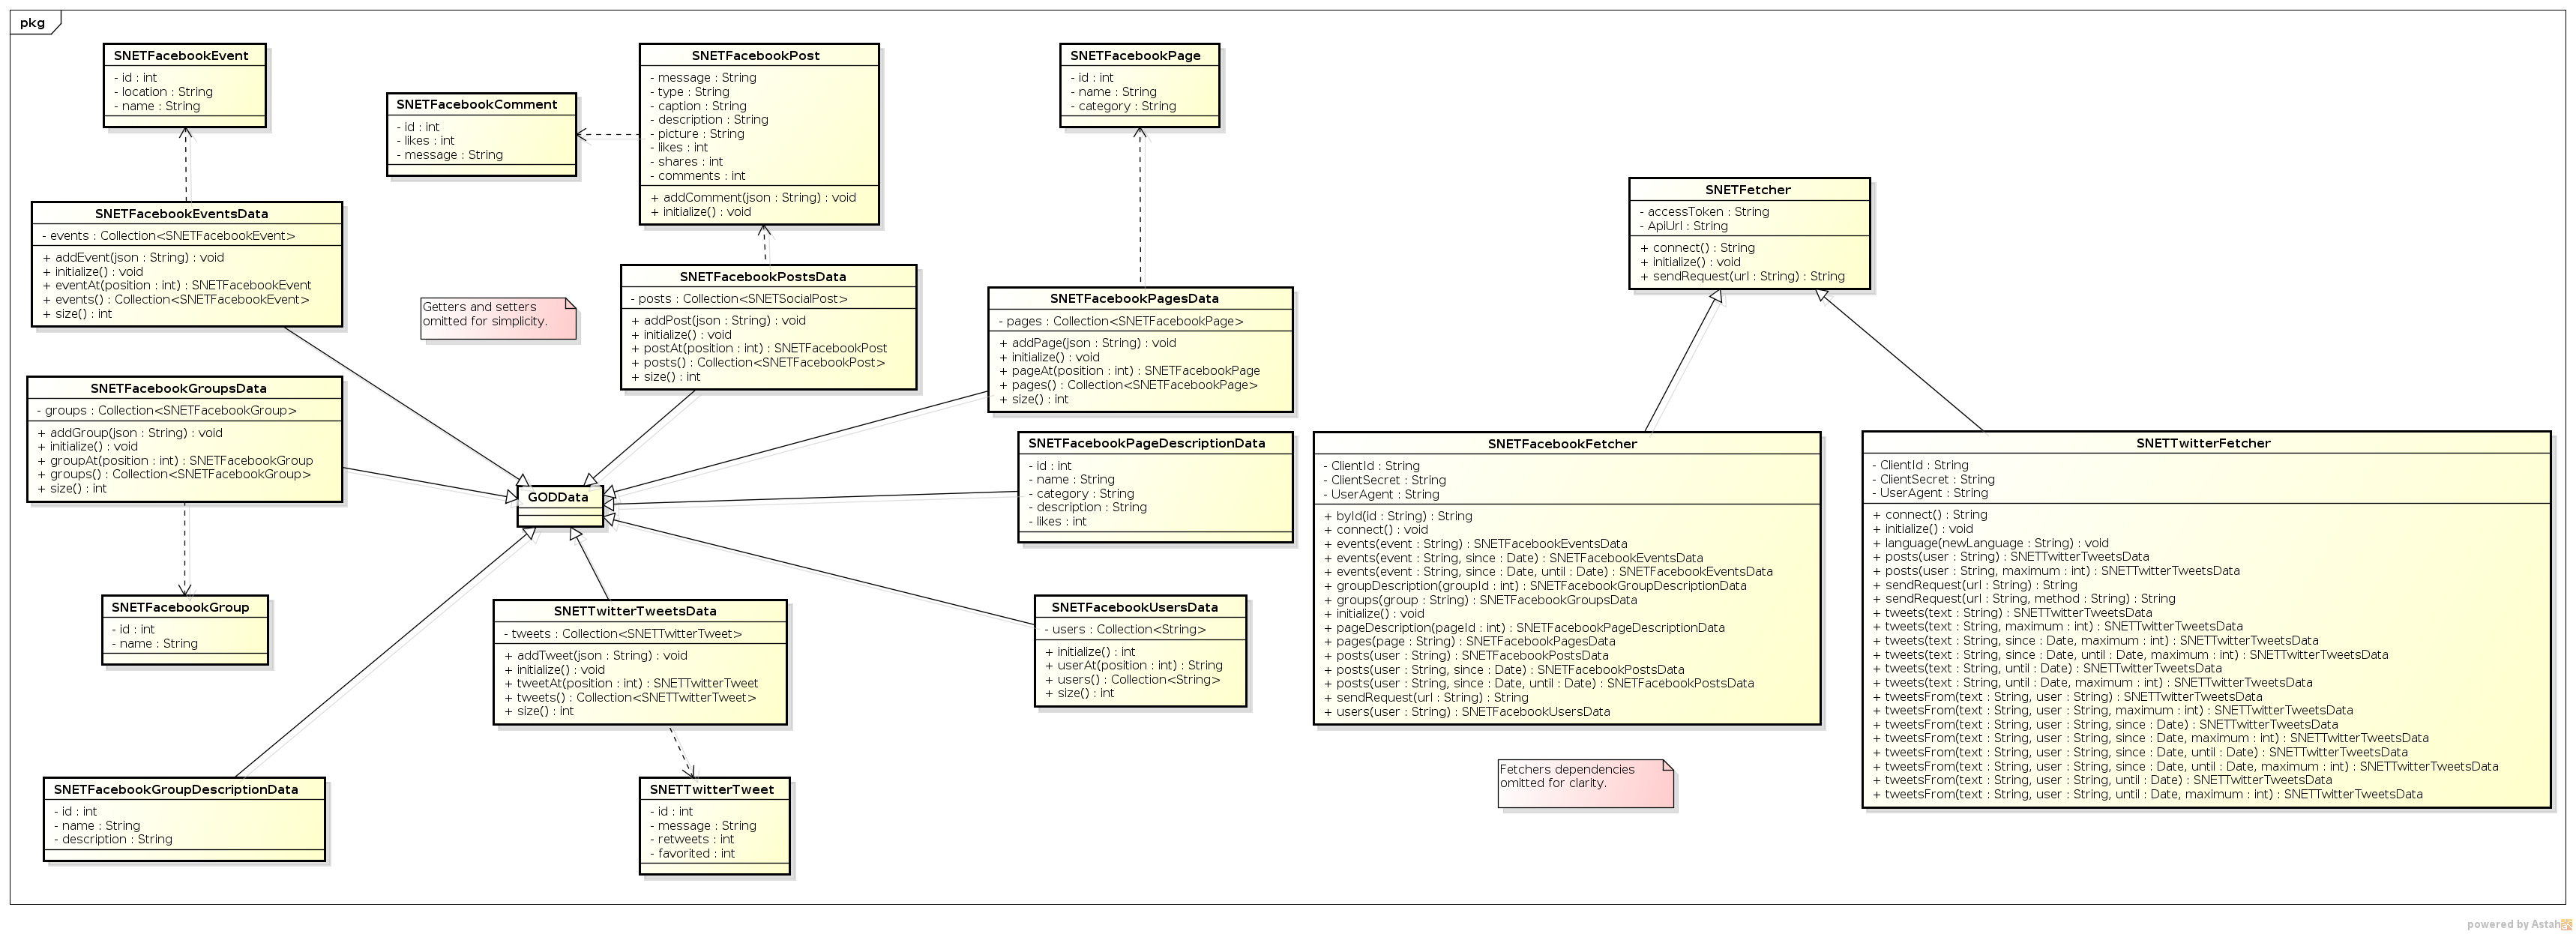
\includegraphics[width=\linewidth]{cd_GODSocialNetIO.png}
\label{fig:cd-godsocialnetio}
\end{figure}

\subsection{Textos (GODTextIO)}
\begin{figure}[H]
\centering
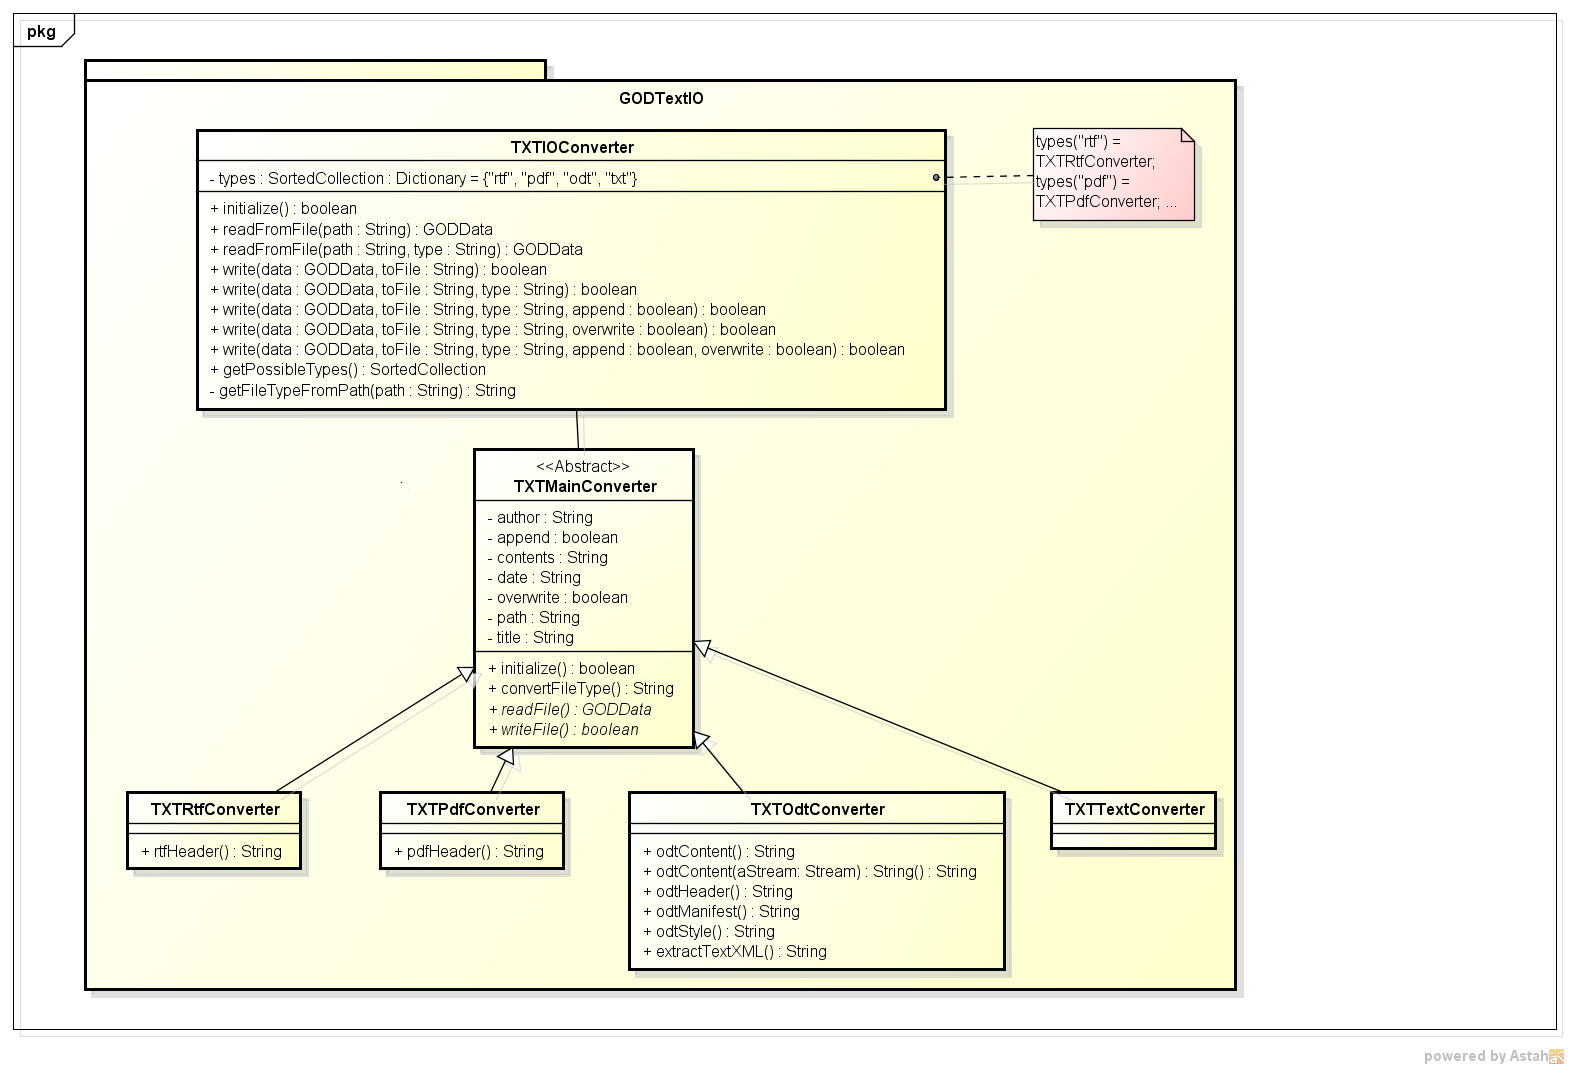
\includegraphics[width=\linewidth]{cd_GODTextIO.png}
\label{fig:cd-godtextio}
\end{figure}

\subsection{Web (GODWeb)}
% \begin{figure}[H]
% \centering
% \includegraphics[width=\linewidth]{cd_GODWeb.png}
% \label{fig:cd-godweb}
% \end{figure}

\subsection{Agregação de conferências (GODAcademics)}
\begin{figure}[H]
\centering
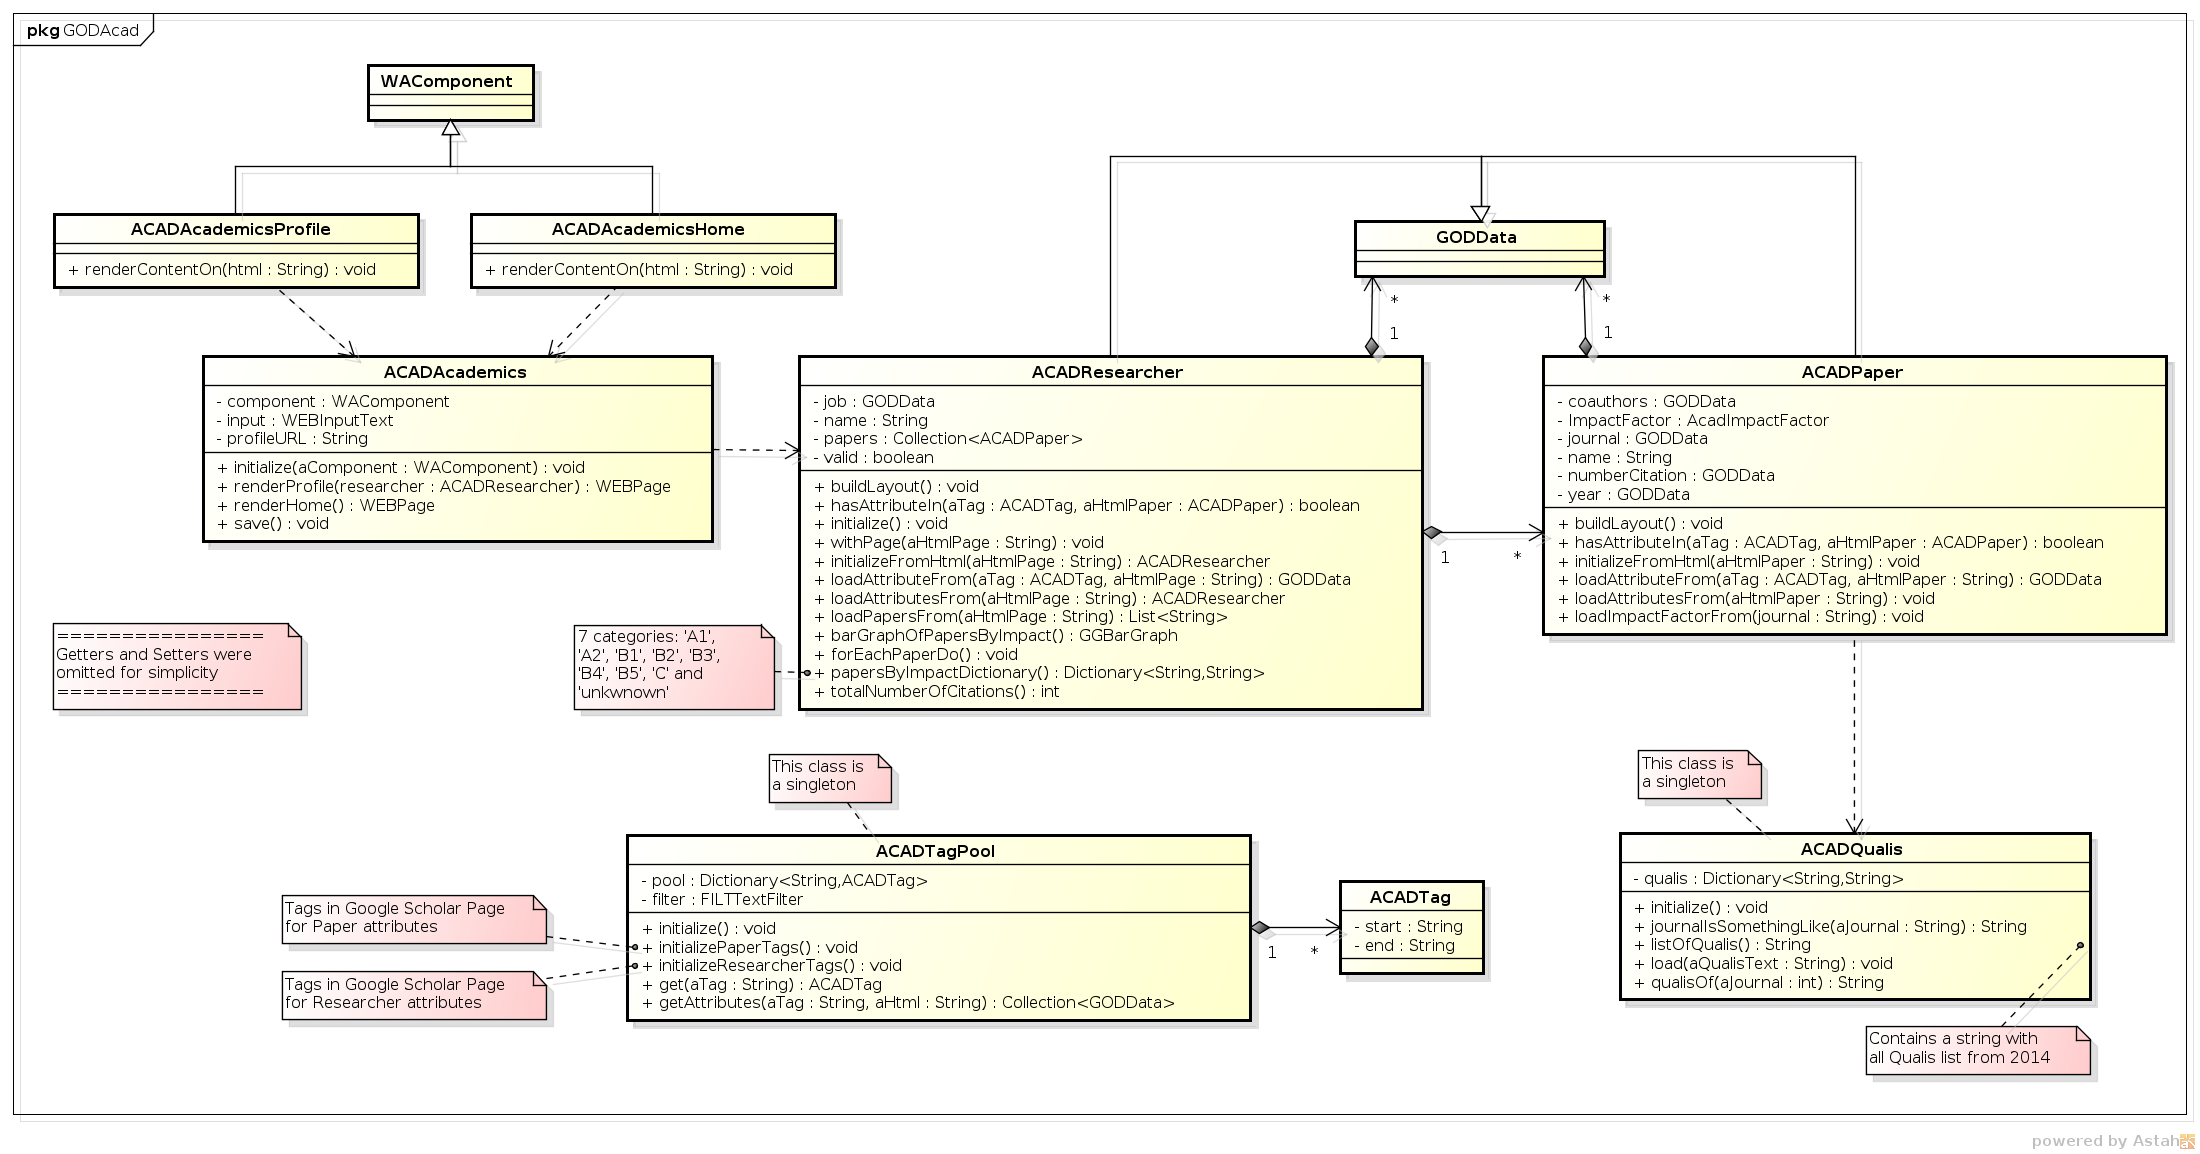
\includegraphics[width=\linewidth]{cd_GODAcademics.png}
\label{fig:cd-godacademics}
\end{figure}

\subsection{Agregação de informações acadêmicas (GODsCall)}
\begin{figure}[H]
\centering
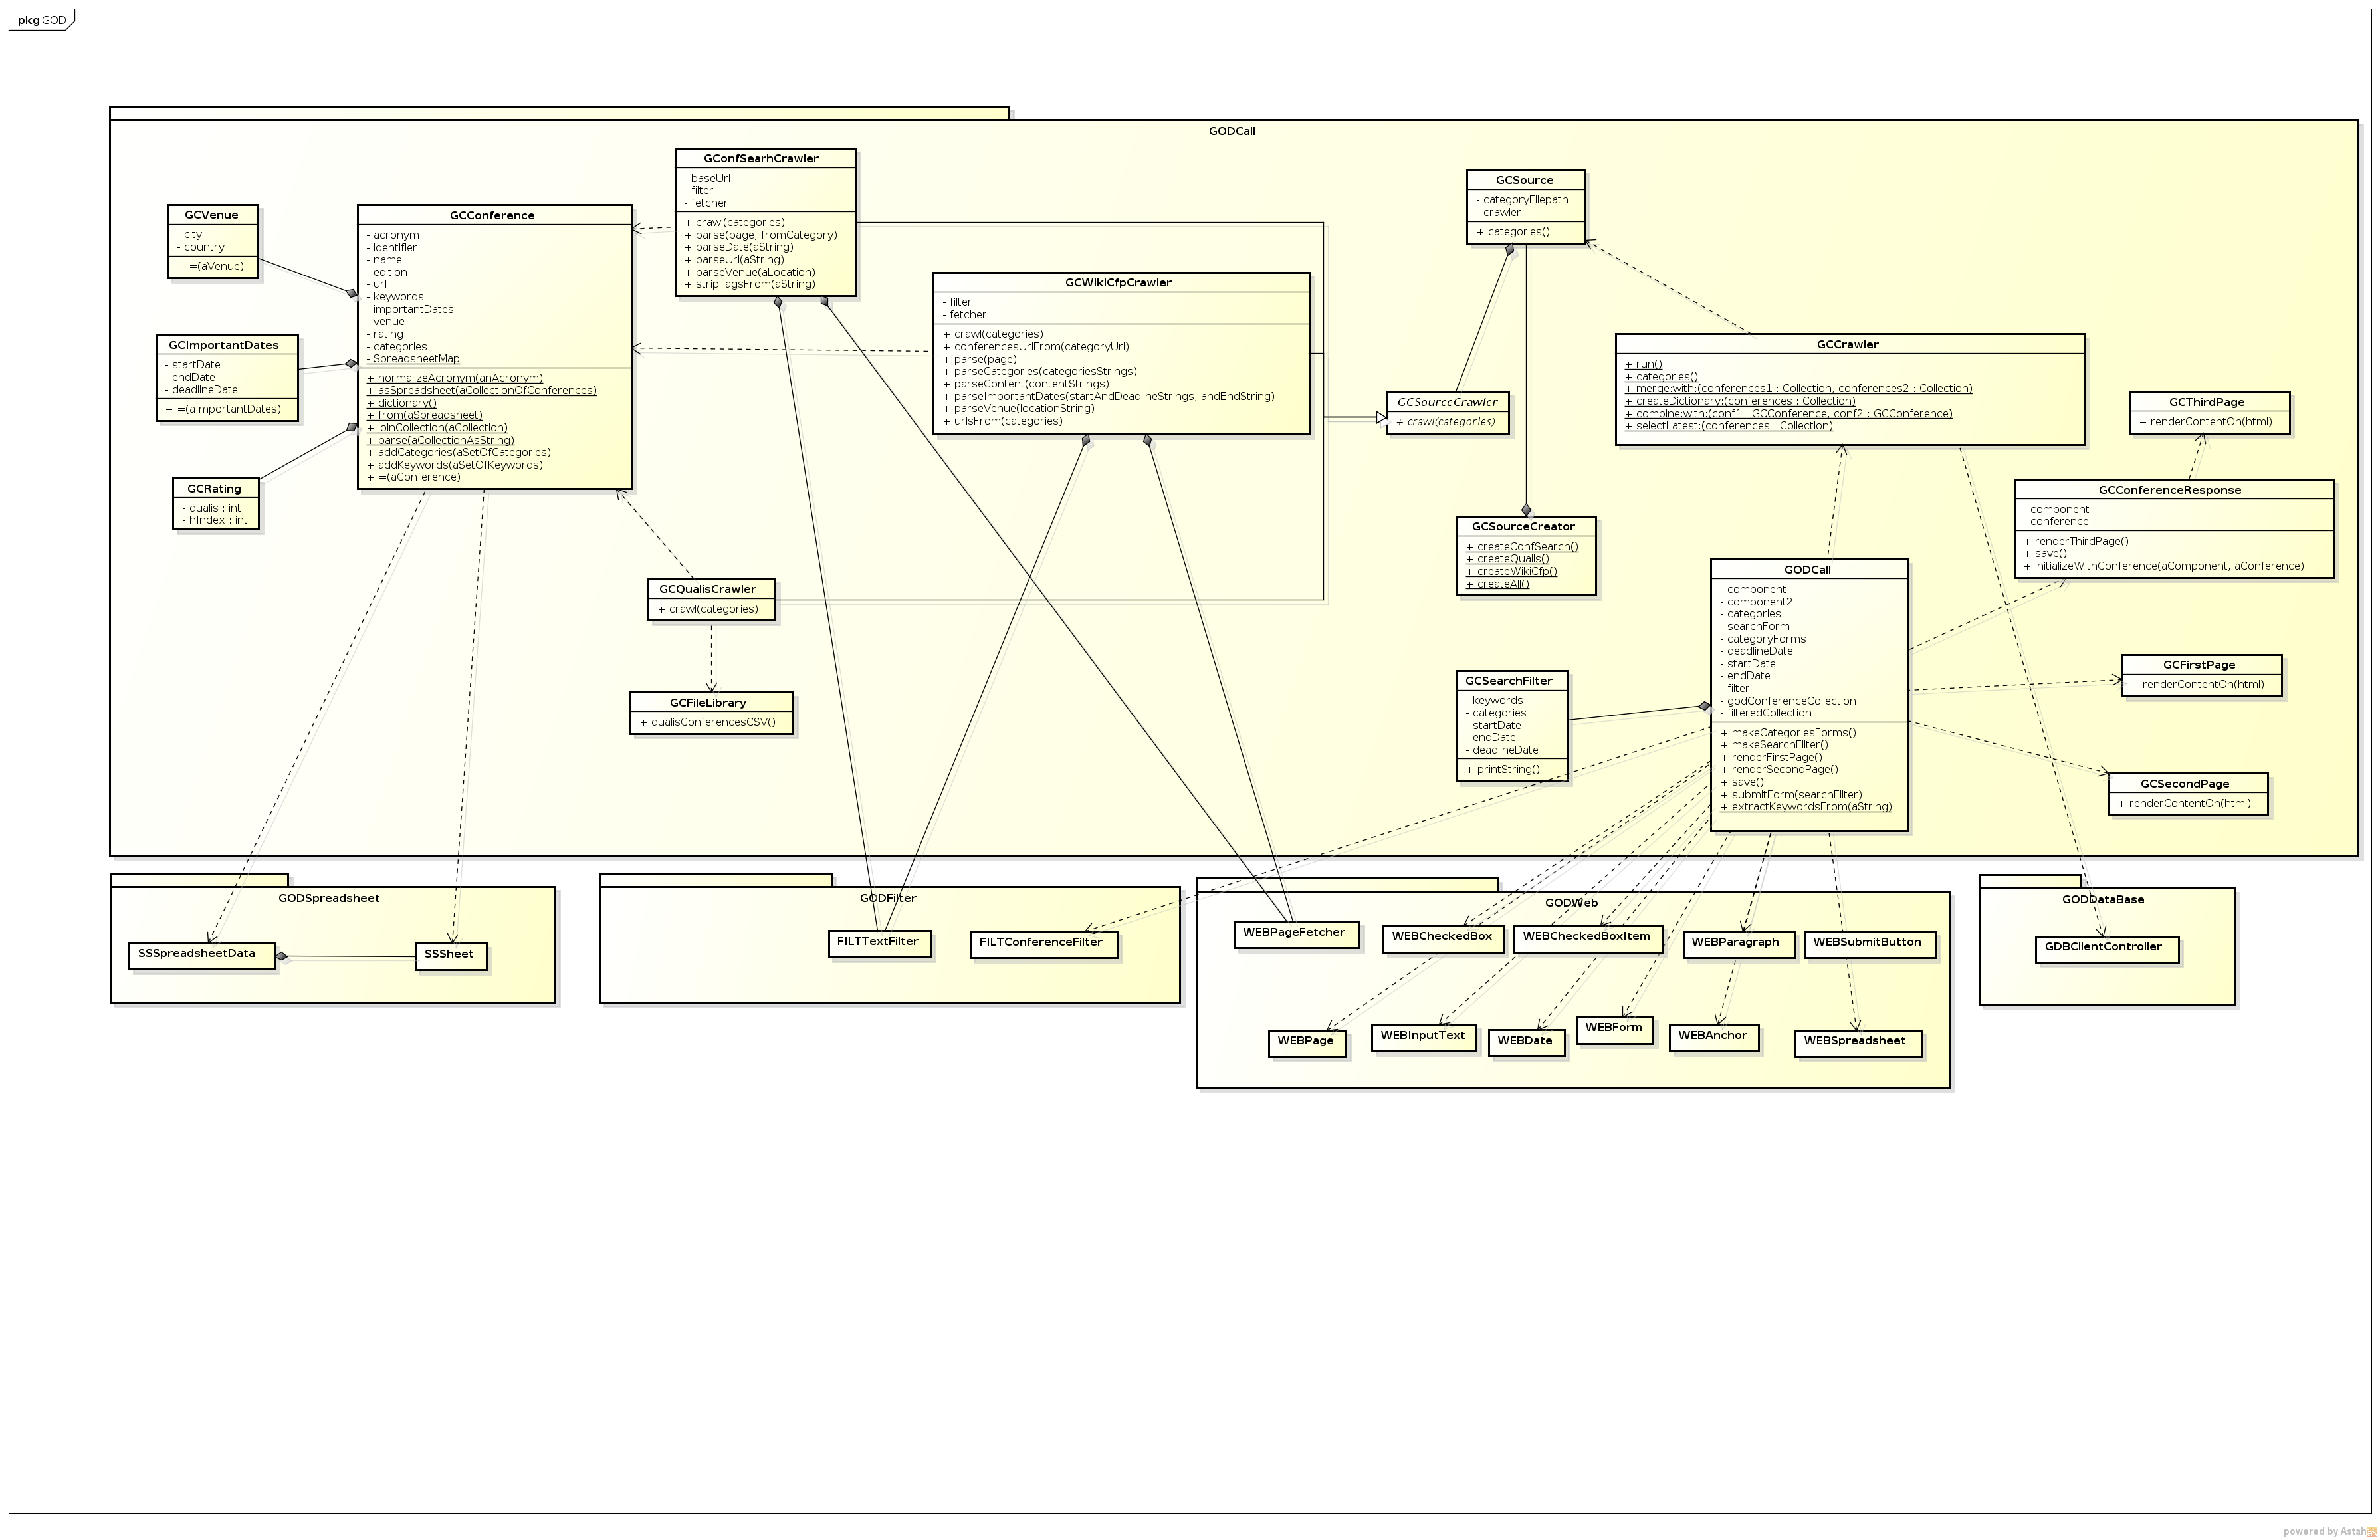
\includegraphics[width=\linewidth]{cd_GODCall.png}
\label{fig:cd-godcall}
\end{figure}

\subsection{Análise de sentimentos de consumo e político (GODSentimentAnalysis)}
\begin{figure}[H]
\centering
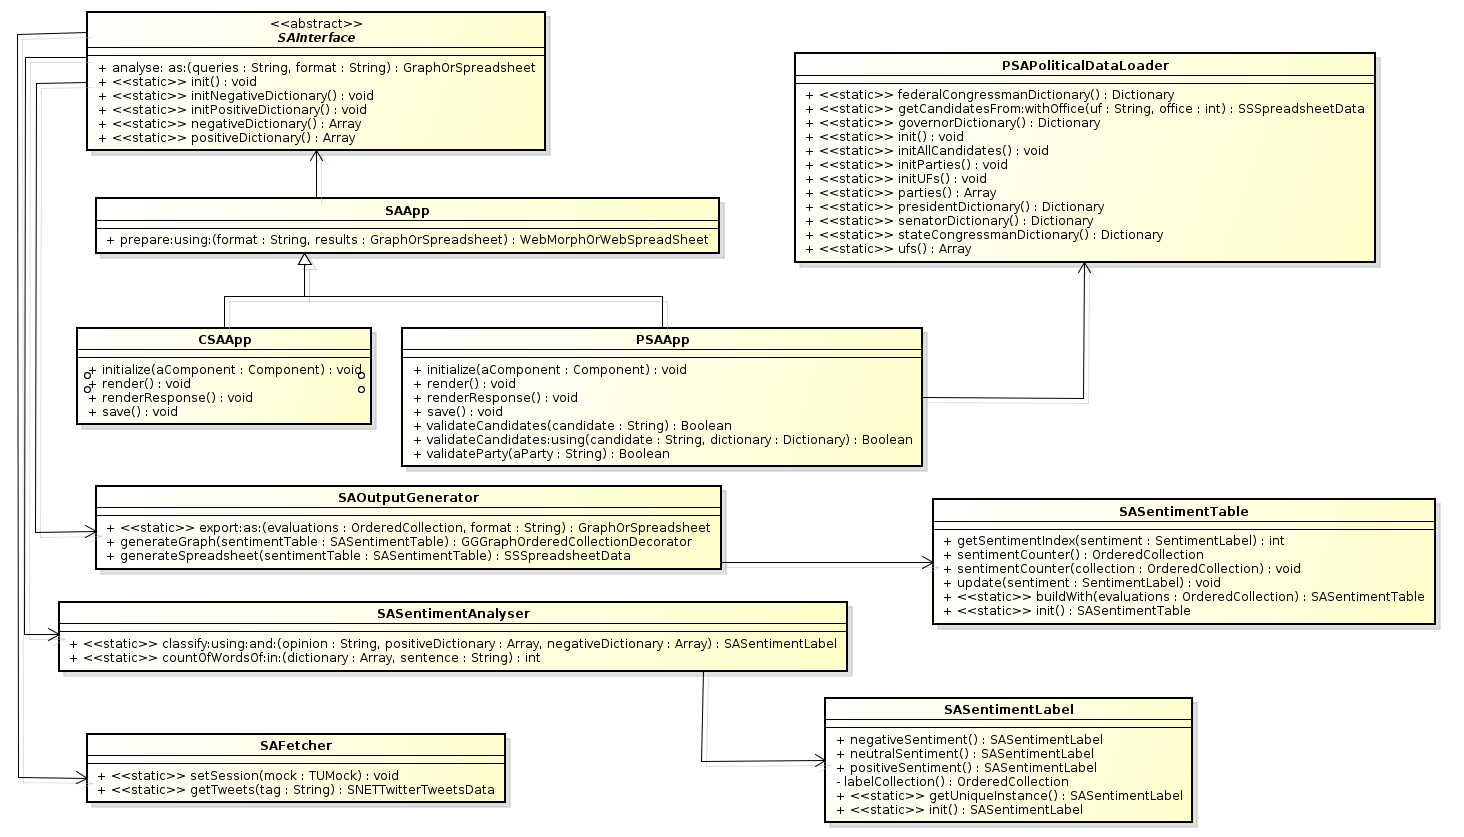
\includegraphics[width=\linewidth]{cd_GODSentimentAnalysis.png}
\label{fig:cd-godsentimentanalysis}
\end{figure}

